\documentclass[a4paper]{article}


\usepackage[utf8]{inputenc}
\usepackage[T1]{fontenc}
\usepackage{textcomp}
\usepackage{mathtools,amssymb,amsthm}
\usepackage[top=2.5cm,bottom=2.5cm,right=2.5cm,left=2.5cm]{geometry}
\usepackage[francais]{babel}
\usepackage{appendix}

%================image=================
\usepackage{graphicx}
\graphicspath{{figures/}}
\renewcommand{\listfigurename}{Table des figures}

%============header and foot============
\usepackage{fancyhdr}
\pagestyle{fancy}
\renewcommand\headrulewidth{1pt}
\fancyhead[L]{\bfseries Programmation Avancée en C}
\fancyhead[R]{
\includegraphics[scale=0.05]{./img_rapport/prepisima.png}}
\fancyfoot[L]{CLIQUOT Théo et CHASSAGNOL Rémi}
\fancyfoot[R]{2020-2021}

%=================other================
\renewcommand{\contentsname}{Table des matières}

%=================code=================
\usepackage{verbatim}
\usepackage{listings}
\usepackage{color}
\usepackage[table]{xcolor}

%==============code settings==========
\definecolor{darkWhite}{rgb}{1,1,1}
\definecolor{myred}{rgb}{1,0.22,0.22}
\definecolor{mypurple}{rgb}{0.74,0.36,0.97}
\lstset{
  mathescape,
  aboveskip=3mm,
  belowskip=-2mm,
  backgroundcolor=\color{darkWhite},
  basicstyle=\ttfamily\footnotesize,
  breakatwhitespace=false,
  breaklines=true,
  captionpos=b,
  commentstyle=\color{myred},
  deletekeywords={...},
  escapeinside={\%*}{*)},
  extendedchars=true,
  framexleftmargin=16pt,
  framextopmargin=3pt,
  framexbottommargin=6pt,
  frame=tb,
  keepspaces=true,
  keywordstyle=\color{mypurple},
  language=C,
  morekeywords={*,...},
  numbers=left,
  numbersep=10pt,
  numberstyle=\tiny\color{black},
  rulecolor=\color{black},
  showspaces=false,
  showstringspaces=false,
  showtabs=false,
  stepnumber=1,
  stringstyle=\color{gray},
  tabsize=4,
  title=\lstname,
}


\begin{document}

\begin{titlepage}


  \begin{figure}[!htb]
    \begin{minipage}{0.5\textwidth}
      \centering
      
\includegraphics[width=.7\linewidth]{./img_rapport/prepisima.png}
      \caption{ ISIMA }\label{fig-ISIMA}
    \end{minipage}\hfill
    \begin{minipage}{0.5\textwidth}
      \centering
      
\includegraphics[width=.7\linewidth]{./img_rapport/logo.png}
      \caption{Université de Clermont-Ferrand}\label{fig-UCA}
    \end{minipage}
  \end{figure}

  \vspace{2cm}

  \begin{center}


    {\huge \bfseries Projet de Programmation avancée en C\\[0.4cm]}

    \vspace{0.5cm}
    
    {\huge Réalisation d'un jeu de Taquin}

    \vspace{1cm}

    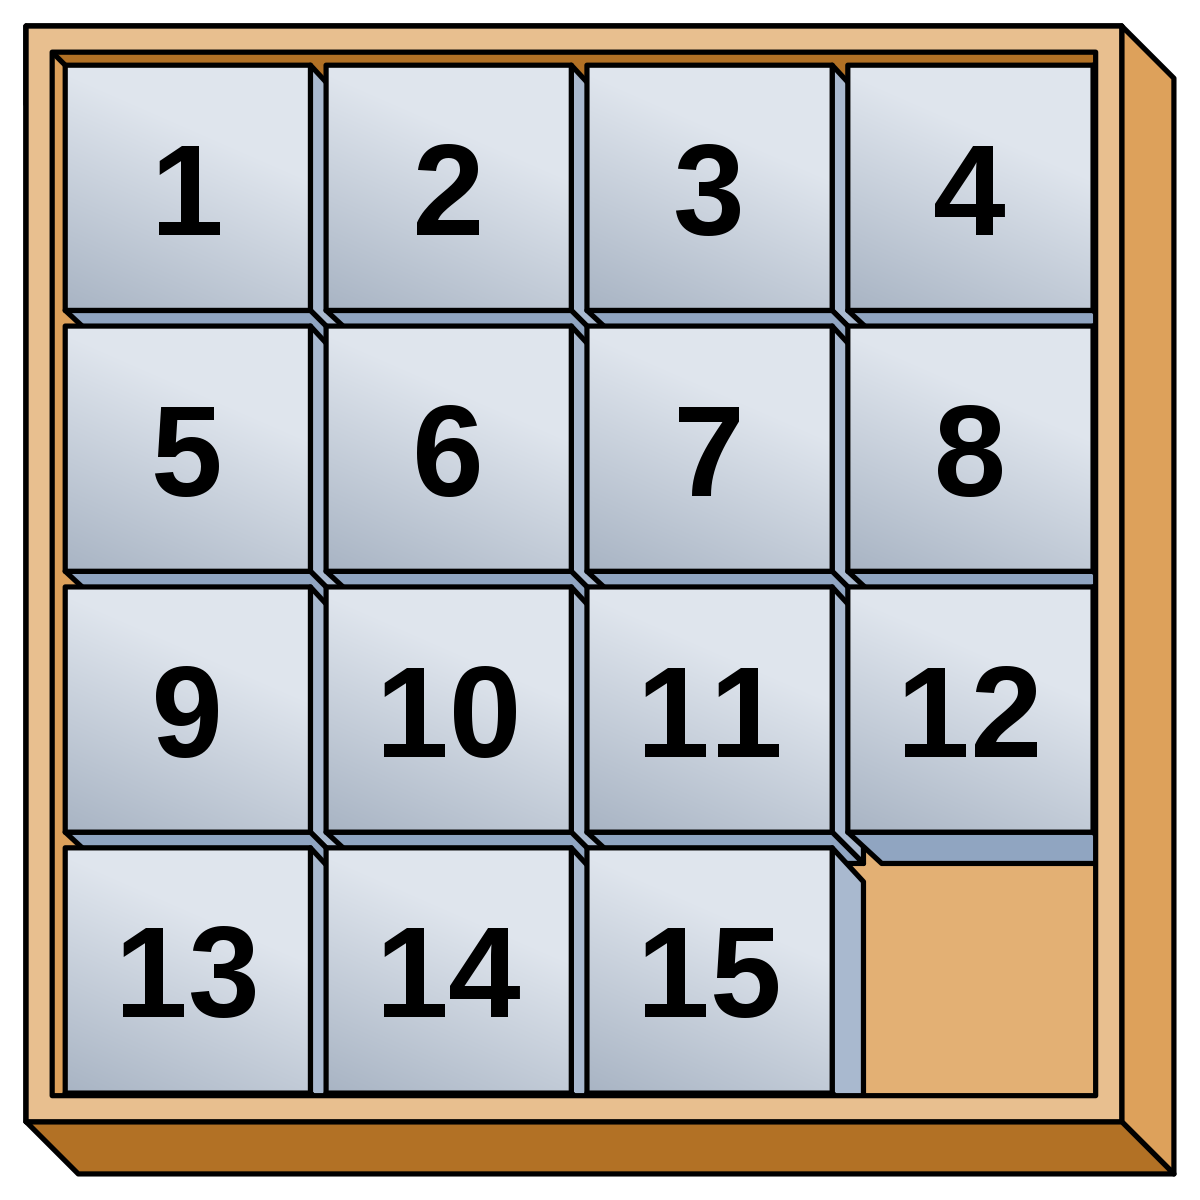
\includegraphics[scale=0.2]{./img_rapport/taquin.png}

    \vspace{1cm}

    \begin{minipage}{0.9\textwidth}
      \begin{flushleft} \large
        CLIQUOT Théo et CHASSAGNOL Rémi\\
        année 2020-2021\\[2cm]
      \end{flushleft}
    \end{minipage}

    \begin{minipage}{0.9\textwidth}
      \begin{flushright} \large
        \emph{Professeurs:} Vincent Limouzy\\
        \emph{Référent TP:} Nicolas Wagner\\
      \end{flushright}
    \end{minipage}

    \vspace{0.5cm}
    
    Travail à rendre pour le : 15/1/2021
    
  \end{titlepage}

  \doublespacing

  \tableofcontents
  \listoffigures

  \doublespacing
  \vspace{2.5cm}

\end{center}

\newpage

\section{Règle du jeux}
\label{sec:regle}


Ce qui va suivre va permettre à n'importe quelle personne de jouer au
taquin. Cette section contient notamment tous les raccourcis clavier et toutes
les fonctionnalités du jeu. Au lancement du jeu, si le joueur exécute le
programme en donnant une grille (fichier texte) en paramètre, il sera affiché le
menu de démarrage, il suffira alors d'appuyer sur une touche du clavier pour
démarrer la partie. Si le joueur ne donne pas de grille, il lui sera d'abord
demandé de saisir dans le terminal la taille de la grille à générer
aléatoirement avant le lancement de l'affichage graphique.

\begin{itemize}
\item Déplacement : Flèches directionnelle ou les touches \texttt{h,j,k,l}.
\item Espace entre les case ou non : touche \texttt{s}.
\item Numéro sur les cases ou non : touche \texttt{n}.
\item Charger un taquin : Pendant l'appel de l'exécutable donné en argument le nom du fichier.
\item Tarquin aléatoire : Lancé l'exécutable sans autre argument (la taille sera demandé via scanf).
\item Tester si le taquin est correcte : touche \texttt{t}
\item Solution au taquin : touche \texttt{r}
\item echap pour l'aide.
\item \texttt{q} pour quitter et sauvegarder si la grille n'est pas trillée.
\end{itemize}


Les mouvements sont définis par rapport à la case vide , c'est à dire que si on à :
\begin{tabular}{|c|c|c|}
  \hline
  5 &  & 10 \\
  \hline
\end{tabular}
et qu'on appui sur $\triangleright$, on obtiendra :
\begin{tabular}{|c|c|c|}
  \hline
  5 & 10 &   \\
  \hline
\end{tabular}
Et inversement si on appui sur $\triangleleft$, on obtiendra :
\begin{tabular}{|c|c|c|}
  \hline
  & 5 & 10  \\
  \hline
\end{tabular}


\section{Fonctionnement}
\label{sec:fonctionnement}

\subsection{Structure du taquin}
\label{subsec:structTaquin}

On utilise la structure suivante (renommée en \texttt{taquin}). \texttt{tab}
correspond à la position de nos pièces par rapport à la grille (un tableau 2D),
l'entier \texttt{posCaseVide} correspond à la position de notre caseVide dans le
taquin (par exemple si il est en bas à droite d'un taquin de dimension 5, il
sera égale à 24), l'entier \texttt{taille} correspond à la dimension du
taquin et enfin, on stocke le nombre de coup effectués par le joueur dans \texttt{nbrCoup}:

\begin{lstlisting}
typedef struct taquin
{
  int ** tab;
  int posCaseVide;
  int taille;
  int nbrCoup;
  
} taquin;
\end{lstlisting}


\subsection{Sauvegarde du taquin}
\label{subsec:sauv}

Cette fonction permet de sauvegarder la grille du joueur dans un fichier nommé
\texttt{sauv\_X.txt} où X est un nombre entier. Pour ce faire, la fonction ouvre
puis ferme tous les fichier \texttt{sauv\_i.txt} jusqu'à tombé sur un fichier
inexistant (le nom n'a pas encore était attribué). Lorsque la fonction trouve le
nom correcte, elle créé le fichier et écrit la grille dedans.

\begin{itemize}
\item Seul le tableau est sauvegardé puisqu'on peut retrouver les autres éléments du taquin à partir de celui-ci.
\item Chaque case du tableau est séparée par un espace.
\item Chaque ligne du tableau est séparée par un saut de ligne.
\end{itemize}

\subsection{Déplacement}
\label{subsec:label}

La fonction de déplacement prend en paramètre le taquin (un pointeur sur la
structure) et un caractère constant qui correspond à la direction choisie. Elle
permute la case vide (de valeur -1) avec la case qui correspond à la pièce que
l'on déplace (qui se situe en haut, en bas, à gauche ou à droite). Si le
mouvement n'existe pas (il n'y a pas de pièce à l'endroit sélectionné par le
joueur), la fonction ne fait rien.

\subsection{création du taquin}
\label{subsec:creaTaquin}

\subsubsection{Taquin aléatoire}
\label{subsubsec:creaAlea}

Pour créer un taquin aléatoire selon une taille donnée, il nous suffit de créer
un taquin avec un tableau comme on le veut à l'arrivée et assigner à
\texttt{posCaseVide} et \texttt{taille} la bonne valeur. Puis on applique un
certain nombre de fois des déplacements aléatoires afin de mélanger le
tableau. A noter que le fait de mélanger le tableau en faisant appel à la
fonction de déplacement assure de la résolubilité de la grille.

\subsubsection{Taquin charger}
\label{subsubsec:charger}

Il nous suffit de lire un fichier avec la même construction que notre fichier de
sauvegarde et récupérer les valeurs de \texttt{tableau}, \texttt{taille} et
\texttt{posCaseVide}

\subsection{Taquin Trié}
\label{subsec:taquinTrié}

Il suffit de parcourir le tableau est de regarder si dans la case 0 on à 1, dans
la case 1 on à 2 ... et pour la dernière -1. Pour cela, la fonction utilise une
boucle \textbf{for} allant de 0 à la taille au carrée - 1 et test si la case de
coordonnées \textbf{(i/taille, i\%taille)} contient la valeur \textbf{i + 1}
puis test si la dernière case du tableau contient -1. La fonction retourne 1 si
la grille est valide, 0 sinon.



% Ma Partie

\section{L'affichage SDL}

Il y a en tout cinq fonctions d'affichage pour cinq écran différents. La
première fonction va afficher le message de début de jeu (et le logo), la
seconde va afficher un message qui demande à l’utilisateur si il souhaite
sauvegarder sa progression dans la partie. Les trois autres vont afficher les
écrans de jeu de fin et le menu d'aide.

\subsection{L'affichage Principal}

Cette fonction est la fonction d'affichage principale, elle va afficher les
différentes parties de l'image en fonction de la grille du taquin. Chaque case du
tableau correspond à une certaine partie de l'image en fonction de la valeur
qu'elle contient. Par exemple, une case qui contient 1 correspond au coin en haut
à gauche de l'image. La taille de la surface de l'image qui correspond à une
case de tableau dépend de la taille de la grille car la taille de l'image est fixe.

Cette fonction utilise une seule surface (sans compter l'écran) qui contient
l'image et deux \textbf{SDL\_Rect}; une qui sert à découper l'image en plusieurs
partie et l'autre qui contient la position de la partie de l'image coller sur l'écran.

\subsection{Les affichages secondaires}
\subsubsection{L'affichage de l'écran de départ}

Cette fonction permet d'afficher le petit texte qui apparaît lorsqu'on lance le
programme. Elle affiche aussi le logo de DOOM en utilisant la fonction
\textbf{SDL\_SerColorKey} et l'option \textbf{SDL\_SRCCOLORKEY} pour ne pas
afficher le fond blanc du logo. Elle fait appel à la fonction \textbf{attend\_touche} pour
attendre que l'utilisateur appui sur une touche pour démarrer le jeu et donc
changer l'affichage. Cette fonction retourne un entier pour que l'on puisse
détecter quand l'utilisateur quitte la fenêtre et donc ne pas démarrer le jeu dans
la fonction main.

\subsubsection{Le menu d'aide}

Cette fonction est appelée quand l'utilisateur appuis sur la touche \textbf{escape}
pendant le jeu et affiche un texte qui donne les différents contrôles clavier au
joueur.

\subsubsection{La demande de sauvegarde}

Cette fonction est appelée quand l'utilisateur quitte la fenêtre (en appuyant
sur \textbf{q}) sans avoir fini le jeu. Elle affiche un texte expliquant que
l'utilisateur peut appuyer sur \textbf{y} pour sauvegarder sa partie, toute
autre touche fermera le programme sans sauvegarde. La boucle attendant la
réponse de l'utilisateur se trouve dans la fonction.

\subsubsection{L'affichage de fin}

Cette fonction est appelée quand l'utilisateur a complété le défi et a appuyé
sur \textbf{t} ou \textbf{q}. Elle affiche ``victoire'' et aussi le nombre de
coup que le joueur a mis pour terminer le jeu à l'aide de \textbf{SDL\_TTF}. Elle fait
appel à la fonction \textbf{attend\_touche} qui permet d'attendre que le joueur
appuis sur une touche pour fermer le programme.

\section{Les contrôles claviers}

Il y a deux fonctions qui permettent de détecter quand l'utilisateur appuis sur
des touches du clavier. La fonction \textbf{attend\_touche} qui est située dans
affichage.c et la fonction \textbf{recup\_touche} située dans le main.c.

\subsection{Fonction principale}

Cette fonction permet de récupérer toutes le entrées clavier qui correspondes à
celles affichées par le menu d'aide pendant la partie (déplacements,
\dots). Elle utilise la fonction \textbf{Wait\_Event} de la library sdl qui
attend une action de l'utilisateur puis qui enregistre cette action dans la
variable \textbf{evenement}. Ensuite, on utilise \textbf{switch} imbriqués, le
premier effectue des action en fonction du type d’avènement (ici seul
\textbf{SDL\_QUIT} et \textbf{SDL\_KEYDOWN} sont utilisé). Le second
\textbf{switch} intervient lorsque l'évènement est de type \texttt{touche
  pressée} et va donc effectuer les actions des différents contrôles clavier
quand la touche pressée correspond. Cette fonction retourne 0 quand
l'utilisateur fait l'action de fermer la fenêtre (ou appui sur \textbf{q}) pour
pouvoir stopper le programme dans le main.

\subsection{Fonction secondaire}

Cette fonction attend que l'utilisateur ferme la fenêtre (et retourne 0 lorsque
c'est le cas) ou appuis sur une touche du clavier, elle permet de maintenir un
affichage tant que l'utilisateur ne fait rien. Elle utilise une boucle
\textbf{while} pour éviter d'être stoppée si \textbf{Wait\_Event} enregistre un
éventement de type différent de \textbf{SDL\_QUIT} ou \textbf{SDL\_KEYDOWN}.

\section{Résolution}

La résolution consiste à réarranger la première ligne, puis la seconde
... jusqu'à ce qu'il nous reste les 2 dernières lignes. Ensuite on va réarranger
les colonnes de taille 2 jusqu'à ce qu'il nous reste qu'un carrée de quatre
cases. Ensuite il nous reste plus qu'à le tourner jusqu'à obtenir le bonne
rotation.

Pour la première étape. On va à chaque fois positionner les cases à leur place
respective sauf pour les cases des deux dernières colonnes. ou on va utiliser
une méthode pour mettre les 2 en même temps sans bloquer la case vide après.

Pour la seconde étape même principe on va utiliser une méthode pour remplir les
2 cases d'une même colonne

Le principe consiste à mettre la case de l'avant dernière colonne (ligne) à la
place de la case de la dernière ligne (colonne). Puis de mettre celle de la
dernière colonne (ligne) en bas (à gauche) de sa position. puis on fait une
boucle.


\end{document}
